\jietitle{1.1 空间向量及其运算}

\xiaojietitle{1.1.1 空间向量及其运算}

本节10题：简单6｜中档4｜难0　提分线：简单→保60\%｜中档→保80\%

\zutit{1.1.1.1 知识讲解｜空间向量及其运算}

1.1.1-1．〔基〕空间向量

\biaoqian{【编注】}与必修2平面向量初步的定义类比记忆（只多``空间''二字）；零向量方向任意、模为0，是概念题易错点。

（1）定义：在空间，我们把具有大小和方向的量叫做空间向量．

（2）长度：空间向量的大小叫做空间向量的长度或模．

\biaoqian{【编注】}对比辨析------空间向量与平面向量（旧知识：必修2第6章平面向量初步）：

\begin{table}[!t]\centering\begin{tabular}{@{}
  >{\raggedright\arraybackslash}p{(\linewidth - 4\tabcolsep) * \real{0.1231}}
  >{\raggedright\arraybackslash}p{(\linewidth - 4\tabcolsep) * \real{0.2051}}
  >{\raggedright\arraybackslash}p{(\linewidth - 4\tabcolsep) * \real{0.6718}}@{}}
\toprule
对比项 & 旧知识：平面向量 & 新知识：空间向量 \\
研究范围 & 同一平面内（二维） & 空间中（三维），平面情形为其特例 \\
定义 & 具有大小和方向的量 & 具有大小和方向的量，含义一致 \\
加减、数乘与数量积 & 三角形／平行四边形法则与运算律 &
法则与运算律完全一致，直接迁移 \\
共线与共面 & 共线向量定理刻画平面内位置关系 &
共线定理（条目5）与共面向量定理（条目9）并用，刻画空间位置关系 \\
易混点 & ------ &
任意两个空间向量必共面，但``不共线''的两向量只张成一张平面，不能作空间基底（须三个不共面，条目10） \\
\bottomrule
\end{tabular}\end{table}

1.1.1-2．〔基〕\textbf{空间向量的表示}

\biaoqian{【编注】}字母表示与有向线段表示贯穿全章书写，解题前先统一记号；模的记号与绝对值区分，避免混淆。

（1）字母表示法：用字母\(\overrightarrow{a},\overrightarrow{b},\overrightarrow{c}, \cdot \cdot \cdot\)，表示．

（2）几何表示法：用有向线段表示，其长度表示空间向量的模．即若向量\emph{a}的起点是\emph{A}，终点是\emph{B}，则向量\(\overrightarrow{a}\)也可以记作\(\overrightarrow{AB}\)，其模记为\(\left| \overrightarrow{a} \right|\)或\(\left| \overrightarrow{AB} \right|\)．

1.1.1-3．〔基〕几类特殊向量

\biaoqian{【编注】}概念辨析高频条目，判定按定义逐条核对；注意共线向量不要求在同一直线上（平行或重合均可），且零向量与任意向量平行（衔接条目5）。

\begin{table}[!t]\centering\begin{tabular}{@{}
  >{\raggedright\arraybackslash}p{(\linewidth - 2\tabcolsep) * \real{0.1666}}
  >{\raggedright\arraybackslash}p{(\linewidth - 2\tabcolsep) * \real{0.8334}}@{}}
\toprule
\begin{minipage}[b]{\linewidth}\raggedright
特殊向量
\end{minipage} & \begin{minipage}[b]{\linewidth}\raggedright
定义
\end{minipage} \\
\midrule
零向量 & 长度为0的向量叫做零向量，记为0 \\
单位向量 & 模为1的向量叫做单位向量 \\
相反向量 &
与\(\overrightarrow{a}\)长度相同而方向相反的向量叫做\(\overrightarrow{a}\)的相反向量，记为\(- \overrightarrow{a}\) \\
共线向量或平行向量 &
若表示若干空间向量的有向线段所在的直线互相平行或重合，那么这些向量叫做共线向量或平行向量；

规定：零向量与任意向量平行．即对任意向量\(\overrightarrow{a}\)，都有\(\overrightarrow{0} \parallel \overrightarrow{a}\) \\
相等向量 & 方向相同且模相等的向量 \\
\bottomrule
\end{tabular}\end{table}

1.1.1-4．〔基〕空间向量的线性运算

\biaoqian{【编注】}全章运算的基础，加减、数乘的法则与运算律均与平面向量一致，类比迁移即可；线性组合的运用见条目9与10。

空间向量的线性运算

\begin{table}[!t]\centering\begin{tabular}{@{}
  >{\raggedright\arraybackslash}p{(\linewidth - 4\tabcolsep) * \real{0.2581}}
  >{\raggedright\arraybackslash}p{(\linewidth - 4\tabcolsep) * \real{0.3952}}
  >{\raggedright\arraybackslash}p{(\linewidth - 4\tabcolsep) * \real{0.3468}}@{}}
\toprule
\begin{minipage}[b]{\linewidth}\raggedright
加法
\end{minipage} & \begin{minipage}[b]{\linewidth}\raggedright
\(\overrightarrow{a} + \overrightarrow{b} = \overrightarrow{OA} + \overrightarrow{AB} =\)\(\overrightarrow{OB}\)
\end{minipage} &
\multirow{2}{=}{\begin{minipage}[b]{\linewidth}\raggedright
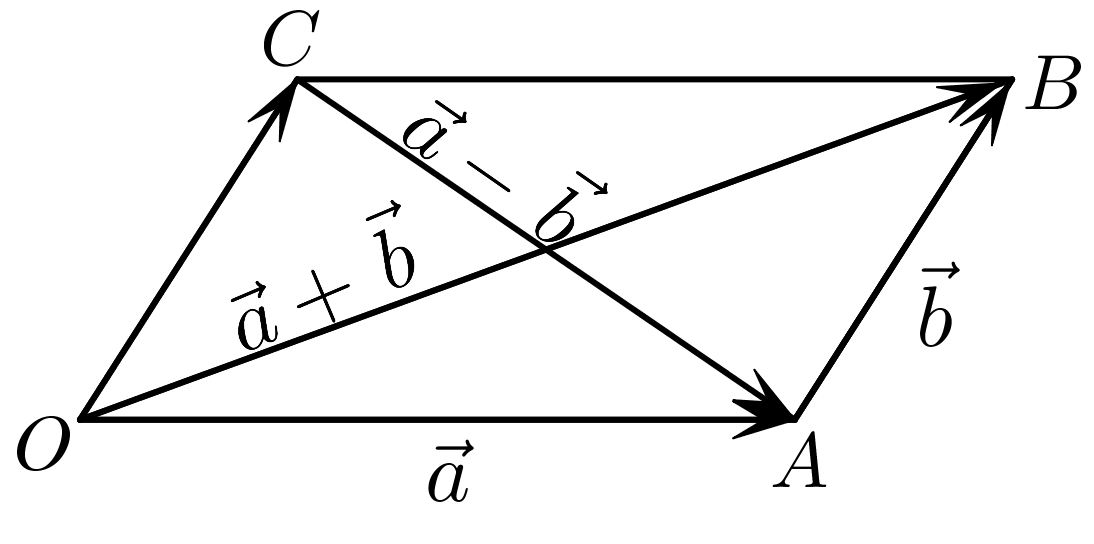
\includegraphics[width=\linewidth,alt={@@@57ceb128-6ced-4fe2-9e22-e16addd5170c}]{media/media/sub3_B_1.png}
\end{minipage}} \\
\begin{minipage}[b]{\linewidth}\raggedright
减法
\end{minipage} & \begin{minipage}[b]{\linewidth}\raggedright
\(\overrightarrow{a} - \overrightarrow{b} = \overrightarrow{OA} - \overrightarrow{OC} =\)\(\overrightarrow{CA}\)
\end{minipage} \\
\midrule
\multirow{3}{=}{数乘运算} &
当\(\lambda > 0\)时，\(\lambda\overrightarrow{a} = \lambda\overrightarrow{OA} = \overrightarrow{PQ}\)
&
\multirow{3}{=}{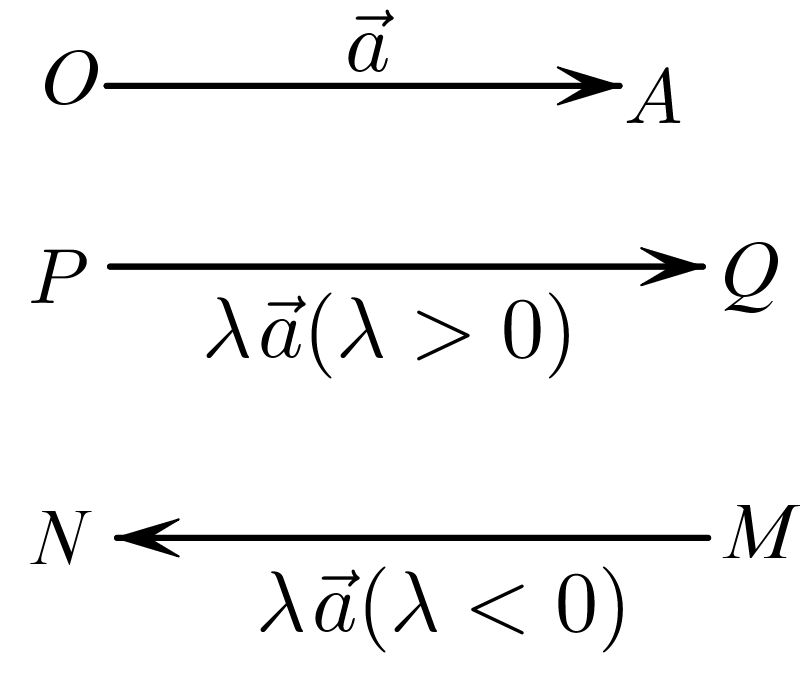
\includegraphics[width=\linewidth,alt={@@@e72cf1b0-1873-4d41-a581-224c31cd9465}]{media/media/sub3_B_2.png}} \\
&
当\(\lambda < 0\)时，\(\lambda\overrightarrow{a} = \lambda\overrightarrow{OA} = \overrightarrow{MN}\) \\
& 当\(\lambda = 0\)时，\(\lambda\overrightarrow{a} = \overrightarrow{0}\) \\
\bottomrule
\end{tabular}\end{table}

运算律

\begin{table}[!t]\centering\begin{tabular}{@{}
  >{\raggedright\arraybackslash}p{(\linewidth - 2\tabcolsep) * \real{0.2157}}
  >{\raggedright\arraybackslash}p{(\linewidth - 2\tabcolsep) * \real{0.7843}}@{}}
\toprule
\begin{minipage}[b]{\linewidth}\raggedright
交换律
\end{minipage} & \begin{minipage}[b]{\linewidth}\raggedright
\(\overrightarrow{a} + \overrightarrow{b} =\)\(\overrightarrow{b} + \overrightarrow{a}\)
\end{minipage} \\
\midrule
结合律 &
\(\left( \overrightarrow{a} + \overrightarrow{b} \right) + \overrightarrow{c} =\)\(\overrightarrow{a} + \left( \overrightarrow{b} + \overrightarrow{c} \right)\)，\(\lambda(\mu\overrightarrow{a}) =\)\((\lambda\mu)\overrightarrow{a}\) \\
分配律 &
\((\lambda + \mu)\overrightarrow{a} = \lambda\overrightarrow{a} + \mu\overrightarrow{a},\lambda(\overrightarrow{a} + \overrightarrow{b}) =\)\(\lambda\overrightarrow{a} + \lambda\overrightarrow{b}\) \\
\bottomrule
\end{tabular}\end{table}

1.1.1-5．〔基〕空间向量共线的充要条件

\biaoqian{【编注】}证线线平行与求参数存在性的基础工具；易错点：与条目9共面充要条件混淆------共线用一个实数、共面用有序实数对。

对任意两个空间向量\(\overrightarrow{a},\overrightarrow{b}(\overrightarrow{b} \neq 0)\)，\(\overrightarrow{a} \parallel \overrightarrow{b}\)的充要条件是存在实数\(\lambda\)，使\(\overrightarrow{a} = \lambda\overrightarrow{b}\)．

1.1.1-6．〔基〕空间向量的夹角

\biaoqian{【编注】}夹角范围（0°到180°）是数量积正负讨论的前提；易混点：几何角（如异面直线所成角）与向量夹角可能互补，运算前先分清求的是哪个角。

\begin{table}[!t]\centering\begin{tabular}{@{}
  >{\raggedright\arraybackslash}p{(\linewidth - 2\tabcolsep) * \real{0.1118}}
  >{\raggedright\arraybackslash}p{(\linewidth - 2\tabcolsep) * \real{0.8882}}@{}}
\toprule
\begin{minipage}[b]{\linewidth}\raggedright
图示
\end{minipage} & \begin{minipage}[b]{\linewidth}\raggedright
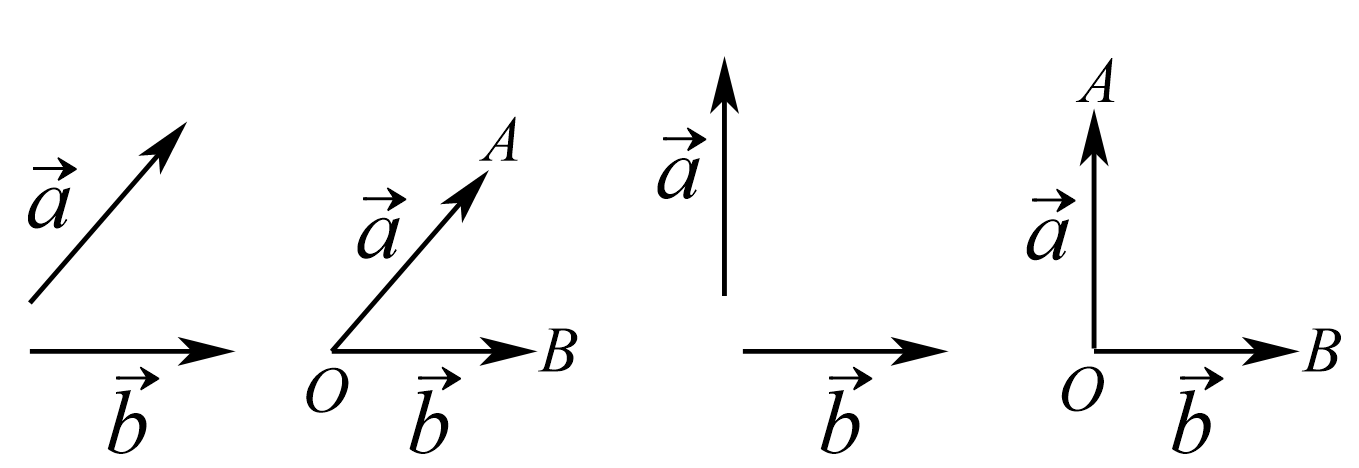
\includegraphics[width=\linewidth,alt={@@@93d04d71-6a01-4600-baaf-bcb9db49ca41}]{media/media/sub3_B_3.png}
\end{minipage} \\
\midrule
定义 &
已知两个非零向量\(\overrightarrow{a}\)，\(\overrightarrow{b}\)，在空间任取一点\emph{O}，作\(\overrightarrow{OA} = \overrightarrow{a}\)，\(\overrightarrow{OB} = \overrightarrow{b}\)，则\(\angle AOB\)叫做向量\(\overrightarrow{a}\)，\(\overrightarrow{b}\)的夹角，记作\(\left\langle \overrightarrow{a},\overrightarrow{b} \right\rangle\) \\
范围 &
通常规定：0\(\leq \langle\overrightarrow{a},\overrightarrow{b}\rangle \leq\)\(\overrightarrow{\pi}\)；

当\(\langle\overrightarrow{a},\overrightarrow{b}\rangle =\)\(\frac{\pi}{2}\)时，\(\overrightarrow{a}\)与\(\overrightarrow{b}\)垂直，记作\(\overrightarrow{a}\bot\overrightarrow{b}\) \\
\bottomrule
\end{tabular}\end{table}

1.1.1-7．〔基〕空间向量的数量积

\biaoqian{【编注】}求空间角与距离的核心运算（支撑条目16、17、34）；注意数量积不满足结合律，零向量与任意向量的数量积为0。

（1）定义：已知两个非零向量\(\overrightarrow{a}\)，\(\overrightarrow{b}\)，则向量\(\overrightarrow{b}\)的模长与\(\overrightarrow{a}\)在向量\(\overrightarrow{b}\)方向上的投影的乘积叫做\(\overrightarrow{a}\)，\(\overrightarrow{b}\)的数量积，记作\(\overrightarrow{a} \cdot \overrightarrow{b}\)．即\(\overrightarrow{a} \cdot \overrightarrow{b} =\)\(|\overrightarrow{a}||\overrightarrow{b}|\cos\langle\overrightarrow{a},\overrightarrow{b}\rangle\)．

\biaoqian{【微提醒】}零向量与任意向量的数量积为0．

（2）由数量积的定义，可以得到：\(\overrightarrow{a}\bot\overrightarrow{b} \Leftrightarrow\)\(\overrightarrow{a} \cdot \overrightarrow{b} = 0\)；\(\overrightarrow{a} \cdot \overrightarrow{a} = |\overrightarrow{a}||\overrightarrow{a}|\cos\langle\overrightarrow{a},\overrightarrow{a}\rangle =\)\({\overrightarrow{a}}^{2}\)．

1.1.1-8．〔基〕投影向量

\biaoqian{【编注】}数量积几何意义的载体，条目33三余弦定理与条目38点面距的推导都基于投影；易错点：投影向量是向量、投影长度是数量。

（1）在空间，向量\(\overrightarrow{a}\)向向量\(\overrightarrow{b}\)投影：

如图①，先将它们平移到同一平面\(\alpha\)内，利用平面上向量的投影，得到与向量\(\overrightarrow{b}\)共线的向量\(\overrightarrow{c}\)，\(\overrightarrow{c} =\)\(\left| \overrightarrow{a} \right|\cos\left\langle \overrightarrow{a},\overrightarrow{b} \right\rangle \cdot \frac{\overrightarrow{b}}{\left| \overrightarrow{b} \right|}\)，称向量\(\overrightarrow{c}\)为向量\(\overrightarrow{a}\)在向量\(\overrightarrow{b}\)上的投影向量．

（2）向量\(\overrightarrow{a}\)在直线\emph{l}上的投影如图②．

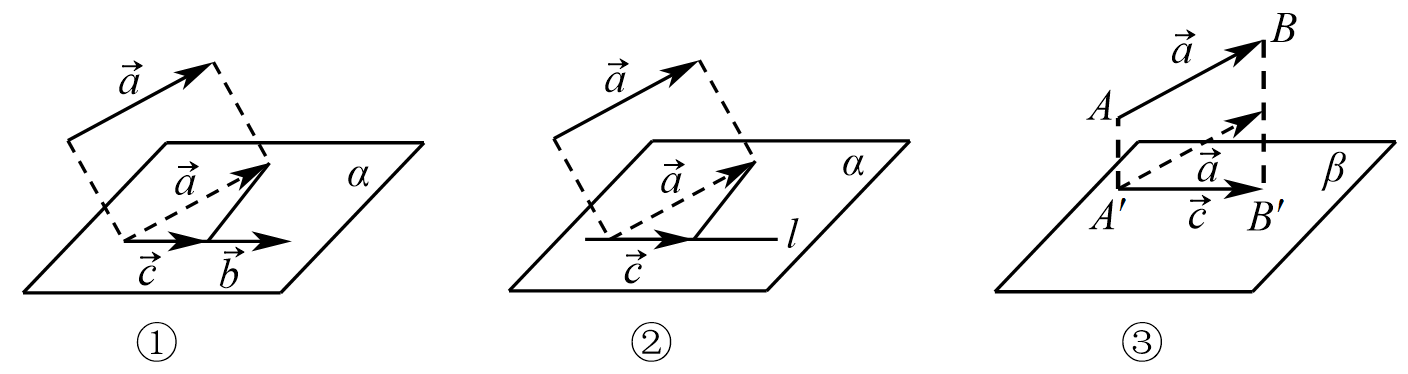
\includegraphics[width=86mm,alt={@@@5da5e1ea-9d33-4579-a56f-804b4a72c894}]{media/media/sub3_B_4.png}

（3）向量\(\overrightarrow{a}\)向平面\(\beta\)投影：

如图③，分别由向量\(\overrightarrow{a}\)的起点\emph{A}和终点\emph{B}作平面\(\beta\)的垂线，垂足分别为\(A'\)，\(B'\)，得到向量\(\overrightarrow{A'B'}\)，向量\(\overrightarrow{A'B'}\)称为向量\(\overrightarrow{a}\)在平面\(\beta\)上的投影向量．

1.1.1-9．〔基〕空间向量共面的充要条件

\biaoqian{【编注】}证四点共面、线共面的标准工具；易错点：定理前提是p与a、b不共线，此前提不可漏，且实数对存在唯一。

（1）共面向量：平行于同一平面的向量，叫做共面向量．

（2）空间向量共面的充要条件：向量\(\overrightarrow{p}\)与不共线向量\(\overrightarrow{a}\)，\(\overrightarrow{b}\)共面的充要条件是存在唯一的有序实数对\((x,y)\)，使\(\overrightarrow{p} =\)\(\overrightarrow{}x\overrightarrow{a} + y\overrightarrow{b}\)．

\zutit{1.1.1.2 空间向量的概念辨析}

1题：-1

\biaoqian{【编注】}题型通式：题干围绕空间向量的模、方向、零向量、单位向量、相等向量与相反向量罗列若干说法要求辨误时，判归本题型。第一步逐条对照定义核验每个说法；再对存疑条目举反例（模相等而方向不同、单位向量方向各异等）；最后排除错误项定答案。

\timu{1.1.1.2-1．（简单）}{下列说法正确的是（~~~~）}

A．若\(\left| \overrightarrow{a} \right| = \left| \overrightarrow{b} \right|\)，则\(\overrightarrow{a} = \overrightarrow{b}\)或\(\overrightarrow{a} = - \overrightarrow{b}\)；B．若\(\overrightarrow{a},\overrightarrow{b}\)为相反向量，则\(\overrightarrow{a} + \overrightarrow{b} = \overrightarrow{0}\)
；C．零向量是没有方向的向量；D．若\(\overrightarrow{a},\overrightarrow{b}\)是两个单位向量，则\(\overrightarrow{a} = \overrightarrow{b}\)

\noindent\biaoqian{【答案】}\ansbox{B}\quad\biaoqian{【知识点】}1.1.1 向量的模、零向量与单位向量、相等向量、相反向量

\biaoqian{【分析】}根据零向量、单位向量、向量的模、相等向量、相反向量等概念逐一分析即可得出答案.

\biaoqian{【详解】}解：若\(\left| \overrightarrow{a} \right| = \left| \overrightarrow{b} \right|\)，则它们的方向相同时是相等向量，方向相反时是相反向量，还有可能方向既不相同，也不相反，A错；

若\(\overrightarrow{a},\overrightarrow{b}\)为相反向量，则它们的和为零向量，B对；

零向量的方向是任意的，C错；

两个单位向量只是模都为1，方向不一定相同，D错.故选：B.

\zutit{1.1.1.3 空间向量的线性运算}

1题：-2

\biaoqian{【编注】}题型通式：题干在几何体中给出若干已知向量、要求用它们表示指定向量时，判归本题型。第一步为目标向量选一条首尾相接的路径写出加减链；再把链中各段用相等或共线的已知向量替换；最后合并化简得表达式。

\timu{1.1.1.3-2．（简单）}{在直三棱柱\(ABC - A_{1}B_{1}C_{1}\)中，若\(\overrightarrow{CA} = \overrightarrow{a},\overrightarrow{CB} = \overrightarrow{b},\overrightarrow{CC_{1}} = \overrightarrow{c},\)，则\(\overrightarrow{A_{1}B}\)=\kongbai.(用\(\overrightarrow{a},\overrightarrow{b},\overrightarrow{c}\)表示)}

\noindent\biaoqian{【答案】}\ansbox{\(\overrightarrow{b} - \overrightarrow{a} - \overrightarrow{c}\)}\quad\biaoqian{【知识点】}1.1.1 棱柱的结构特征和分类、空间向量加减运算的几何表示

\biaoqian{【分析】}连接\(CA_{1},\)根据直三棱柱的结构特征及空间向量减法的几何意义可得\(\overrightarrow{A_{1}B} = \overrightarrow{CB} - \overrightarrow{CA} - \overrightarrow{CC_{1}}\)，结合已知即可求表达式.

\biaoqian{【详解】}连接\(CA_{1},\)则\(\overrightarrow{A_{1}B} = \overrightarrow{CB} - \overrightarrow{CA_{1}} = \overrightarrow{CB} - \overrightarrow{CA} - \overrightarrow{CC_{1}} =\)
\(\overrightarrow{b} - \overrightarrow{a} - \overrightarrow{c}\).

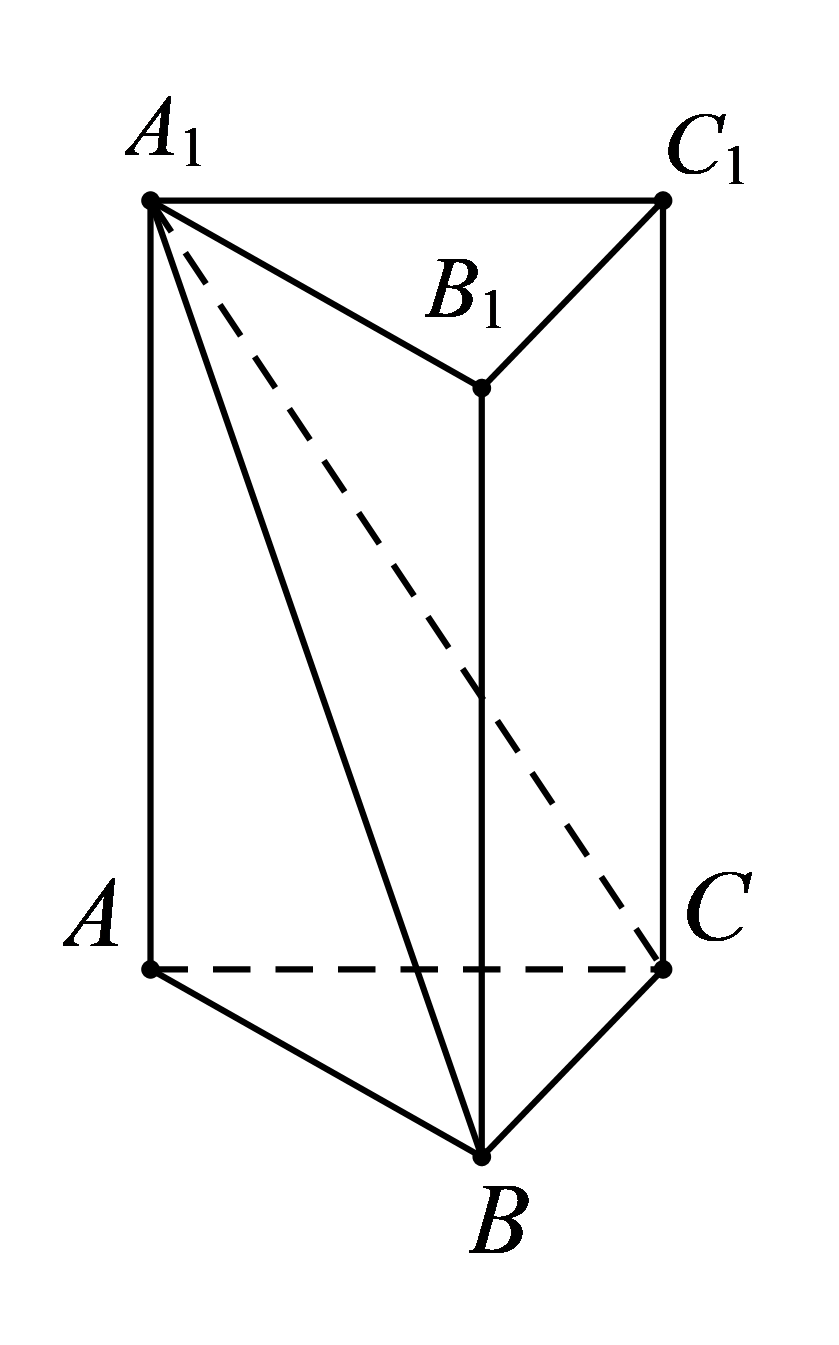
\includegraphics[width=45mm,alt={@@@4e3aa752498e415b9cc3d6d60f7bb3fe}]{media/media/image1.png}

故答案为：\(\overrightarrow{b} - \overrightarrow{a} - \overrightarrow{c}\)

\zutit{1.1.1.4 用基底表示向量}

1题：-3

\biaoqian{【编注】}题型通式：题干指定三个不共面的向量作基底、要求把目标向量写成基底的线性组合并求系数时，判归本题型。第一步把目标向量沿几何路径分解到基向量方向；再把各段按比例关系代入基底；最后比较等式两边系数求出待定值。

\timu{1.1.1.4-3．（简单）}{已知正方体\emph{ABCD}－\emph{A\textsubscript{1}B\textsubscript{1}C\textsubscript{1}D\textsubscript{1}}中，\(\overrightarrow{A_{1}E}\)＝\(\frac{1}{4}\) \(\overrightarrow{A_{1}C_{1}}\)，若\(\overrightarrow{AE} =\)\emph{x}\(\overrightarrow{AA_{1}}\)＋\emph{y}(\(\overrightarrow{AB}\)＋\(\overrightarrow{AD}\))，则\emph{x}＝\kongbai，\emph{y}＝\kongbai.}

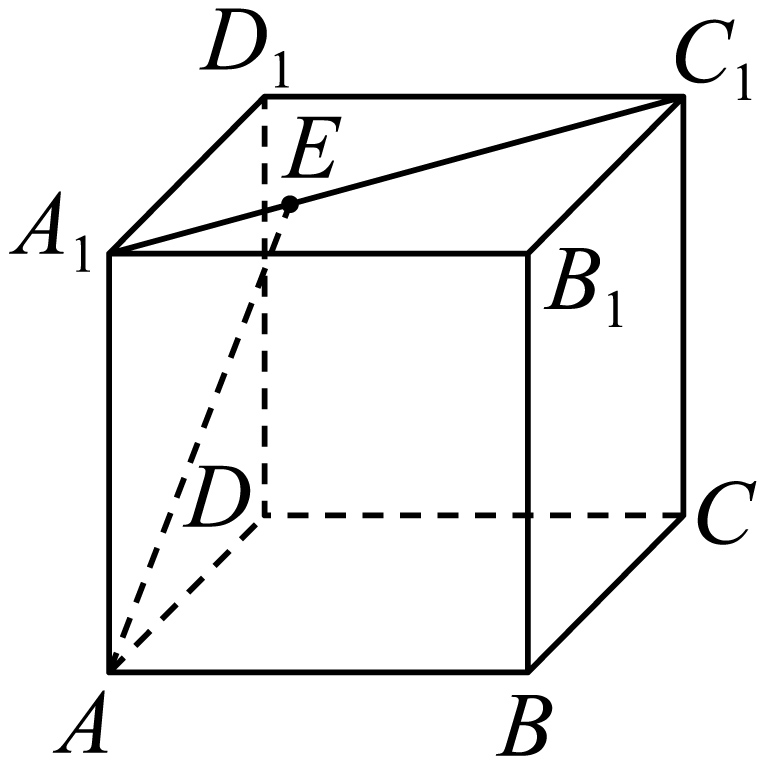
\includegraphics[width=45mm,alt={@@@b0b55c9f-4634-4bba-b096-bc6dd0cf7747}]{media/media/image2.png}

\noindent\biaoqian{【答案】}\ansbox{1 \(\frac{1}{4}\)}\quad\biaoqian{【知识点】}1.1.1 空间向量的加减运算、空间向量的数乘运算、用空间基底表示向量

\biaoqian{【分析】}结合空间向量的线性运算列方程，由此求得\(x,y\)的值.

\biaoqian{【详解】}\(\overrightarrow{AE} = \overrightarrow{AA_{1}} + \overrightarrow{A_{1}E} = \overrightarrow{AA_{1}} + \frac{1}{4}\overrightarrow{A_{1}C_{1}} = \overrightarrow{AA_{1}} + \frac{1}{4}\left( \overrightarrow{AB} + \overrightarrow{AD} \right)\)，所以\(x = 1,y = \frac{1}{4}\).故答案为：\(1\)；\(\frac{1}{4}\)

\zutit{1.1.1.5 共面向量的判定}

1题：-4

\biaoqian{【编注】}题型通式：题干给出 p=xa+yb 或 MP=xMA+yMB
一类线性表示与"共面"结论的互推说法判断时，判归本题型。第一步核对充要条件的前提（两向量不共线或三点不共线）是否齐备；再对缺前提的说法举共线反例排除；最后汇总正确序号定选项。

\timu{1.1.1.5-4．（简单）}{有下列说法:}

①若\(\overrightarrow{p} = x\overrightarrow{a} + y\overrightarrow{b}\)，则\(\overrightarrow{p}\)与\(\overrightarrow{a}\)，\(\overrightarrow{b}\)共面；②若\(\overrightarrow{p}\)与\(\overrightarrow{a}\)，\(\overrightarrow{b}\)共面，则\(\overrightarrow{p}\)=\emph{x}\(\overrightarrow{a}\)+\emph{y}\(\overrightarrow{b}\)；③若\(\overrightarrow{MP}\)=\emph{x}\(\overrightarrow{MA}\)+\emph{y}\(\overrightarrow{MB}\)，则\emph{P}，\emph{M}，\emph{A}，\emph{B}共面；④若\emph{P}，\emph{M}，\emph{A}，\emph{B}共面，则\(\overrightarrow{MP}\)=\emph{x}\(\overrightarrow{MA}\)+\emph{y}\(\overrightarrow{MB}\).其中正确的是（~~~~）

A．①②③④；B．①③④；C．①③；D．②④

\noindent\biaoqian{【答案】}\ansbox{C}\quad\biaoqian{【知识点】}1.1.1 判定空间向量共面

\biaoqian{【分析】}利用空间向量共面定理逐一判断即可.

\biaoqian{【详解】}若\(\overrightarrow{a}\)，\(\overrightarrow{b}\)共线，由\(\overrightarrow{p}\)=\emph{x}\(\overrightarrow{a}\)+\emph{y}\(\overrightarrow{b}\)知\(\overrightarrow{p}\)一定与\(\overrightarrow{a}\)，\(\overrightarrow{b}\)共面，

若\(\overrightarrow{a}\)，\(\overrightarrow{b}\)不共线，则满足共面定理，\(\overrightarrow{p}\)与\(\overrightarrow{a}\)，\(\overrightarrow{b}\)共面，①对；

同理③对；若\(\overrightarrow{p}\)与\(\overrightarrow{a}\)，\(\overrightarrow{b}\)共面，且\(\overrightarrow{a}\)，\(\overrightarrow{b}\)共线，则不一定有\(\overrightarrow{p}\)=\emph{x}\(\overrightarrow{a}\)+\emph{y}\(\overrightarrow{b}\)，故②不对；同理④不对，故选：C.

\zutit{1.1.1.6 数量积的概念与运算律}

1题：-5

\biaoqian{【编注】}题型通式：题干列出数量积相关的若干等式（平方、商式、乘积展开）要求判断正误时，判归本题型。第一步按定义
a·b=\textbar a\textbar\textbar b\textbar cosθ
逐式展开核验；再警惕向量无除法、数量积无结合律等误用；最后汇总正确式定选项。

\timu{1.1.1.6-5．（简单）}{设\(\overrightarrow{a}\)，\(\overrightarrow{b}\)为空间中的任意两个非零向量，下列各式中正确的有（~~~~）}

A．\({\overrightarrow{a}}^{2} = \left| \overrightarrow{a} \right|^{2}\)；B．\(\frac{\overrightarrow{a} \cdot \overrightarrow{b}}{\overrightarrow{a} \cdot \overrightarrow{a}} = \frac{\overrightarrow{b}}{\overrightarrow{a}}\)；C．\(\left( \overrightarrow{a} \cdot \overrightarrow{b} \right)^{2} = {\overrightarrow{a}}^{2} \cdot {\overrightarrow{b}}^{2}\)；D．\(\left( \overrightarrow{a} - \overrightarrow{b} \right)^{2} = {\overrightarrow{a}}^{2} - 2\overrightarrow{a} \cdot \overrightarrow{b} + {\overrightarrow{b}}^{2}\)

\noindent\biaoqian{【答案】}\ansbox{AD}\quad\biaoqian{【知识点】}1.1.1 空间向量数量积的概念辨析、求空间向量的数量积

\biaoqian{【分析】}根据空间向量数量积的定义与运算律一一判断即可；

\biaoqian{【详解】}解：对于A：\({\overrightarrow{a}}^{2} = \overrightarrow{a} \cdot \overrightarrow{a} = \left| \overrightarrow{a} \right| \cdot \left| \overrightarrow{a} \right|\cos 0 = \left| \overrightarrow{a} \right|^{2}\)，故A正确；

对于B：因为向量不能做除法，即\(\frac{\overrightarrow{b}}{\overrightarrow{a}}\)无意义，故B错误；

对于C：\(\left( \overrightarrow{a} \cdot \overrightarrow{b} \right)^{2} = \left( \left| \overrightarrow{a} \right| \cdot \left| \overrightarrow{b} \right|\cos\left\langle \overrightarrow{a},\overrightarrow{b} \right\rangle \right)^{2} = \left| \overrightarrow{a} \right|^{2} \cdot \left| \overrightarrow{b} \right|^{2}\cos^{2}\left\langle \overrightarrow{a},\overrightarrow{b} \right\rangle\)，故C错误；

对于D：\(\left( \overrightarrow{a} - \overrightarrow{b} \right)^{2} = \left( \overrightarrow{a} - \overrightarrow{b} \right) \cdot \left( \overrightarrow{a} - \overrightarrow{b} \right) = {\overrightarrow{a}}^{2} - 2\overrightarrow{a} \cdot \overrightarrow{b} + {\overrightarrow{b}}^{2}\)，故D正确；故选：AD

\zutit{1.1.1.7 数量积求夹角与投影（非坐标法）}

1题：-6

\biaoqian{【编注】}题型通式：题干在几何体中求两向量的夹角、模长或投影而不建坐标系时，判归本题型。第一步平移向量使共起点或选不共面的三个向量作基底；再把相关向量用基底表示并算出数量积与模长；最后代入夹角公式并按向量夹角范围
{[}0,π{]} 取角。

\timu{1.1.1.7-6．（中档）}{如图，在正方体\(ABCD - A_{1}B_{1}C_{1}D_{1}\)中，求向量\(\overrightarrow{BC_{1}}\)与\(\overrightarrow{AC}\)的夹角的大小．}

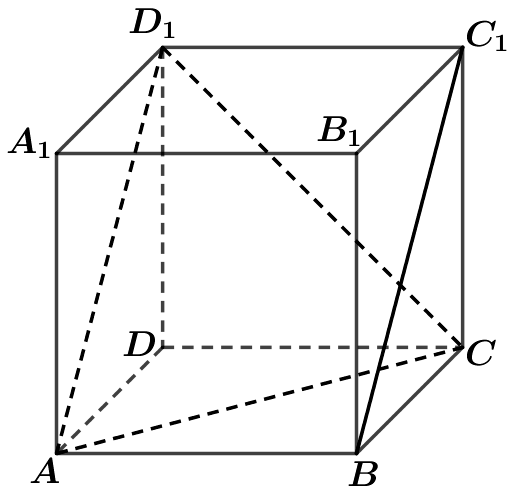
\includegraphics[width=86mm,alt={@@@d8ffc038-cfd6-4d16-b846-f3d81f29b325}]{media/media/image3.png}

\noindent\biaoqian{【答案】}\ansbox{\(60{^\circ}\)}\quad\biaoqian{【知识点】}1.1.1 空间向量数量积的应用

\biaoqian{【分析】}方法1：结合图形，平移向量，利用空间向量的夹角定义来求，但要注意向量夹角的范围；

方法2：先求\(\overrightarrow{BC_{1}} \cdot \overrightarrow{AC}\)，再利用公式\(\cos\left\langle \overrightarrow{BC_{1}},\overrightarrow{AC} \right\rangle = \frac{\overrightarrow{BC_{1}} \cdot \overrightarrow{AC}}{\left| \overrightarrow{BC_{1}} \right| \cdot \left| \overrightarrow{AC} \right|}\)求\(\cos\left\langle \overrightarrow{BC_{1}},\overrightarrow{AC} \right\rangle\)，最后确定\(\left\langle \overrightarrow{BC_{1}},\overrightarrow{AC} \right\rangle\)即可．

\biaoqian{【详解】}解：方法1：因为\(\overrightarrow{AD_{1}} = \overrightarrow{BC_{1}}\)，所以\(\angle CAD_{1}\)的大小就等于\(\left\langle \overrightarrow{BC_{1}},\overrightarrow{AC} \right\rangle\)

因为△\(CAD_{1}\)为等边三角形，所以\(\angle CAD_{1} = 60^{{^\circ}}\)，所以\(\overrightarrow{BC_{1}}\)与\(\overrightarrow{AC}\)的夹角的大小为\(60{^\circ}\)．

方法2．设正方体的棱长为1，\(\overrightarrow{BC_{1}} \cdot \overrightarrow{AC} = \left( \overrightarrow{BC} + \overrightarrow{CC_{1}} \right) \cdot \left( \overrightarrow{AB} + \overrightarrow{BC} \right) = \left( \overrightarrow{AD} + \overrightarrow{AA_{1}} \right) \cdot \left( \overrightarrow{AB} + \overrightarrow{AD} \right)\)\(= \overrightarrow{AD} \cdot \overrightarrow{AB} + \left| \overrightarrow{AD} \right|^{2} + \overrightarrow{AA_{1}} \cdot \overrightarrow{AB} + \overrightarrow{AA_{1}} \cdot \overrightarrow{AD} = 0 + \left| \overrightarrow{AD} \right|^{2} + 0 + 0 = \left| \overrightarrow{AD} \right|^{2} = 1\)又因为\(\left| \overrightarrow{BC_{1}} \right| = \sqrt{2},\left| \overrightarrow{AC} \right| = \sqrt{2}\)，所以\(\cos\left\langle \overrightarrow{BC_{1}},\overrightarrow{AC} \right\rangle = \frac{\overrightarrow{BC_{1}} \cdot \overrightarrow{AC}}{\left| \overrightarrow{BC_{1}} \right| \cdot \left| \overrightarrow{AC} \right|} = \frac{1}{\sqrt{2} \times \sqrt{2}} = \frac{1}{2}\)，
因为\(\left\langle \overrightarrow{BC_{1}},\overrightarrow{AC} \right\rangle \in \lbrack 0,\pi\rbrack\)，所以\(\overrightarrow{BC_{1}}\)与\(\overrightarrow{AC}\)的夹角的大小为\(60{^\circ}\)．

\zutit{1.1.1.8 数量积条件求参（夹角与垂直）}

2题：-7～8

\biaoqian{【编注】}题型通式：题干给出两向量的模与夹角、并以夹角为锐角/钝角或两向量垂直为条件求参数时，判归本题型。第一步用数量积把条件翻译成不等式或方程（锐角\textgreater0、钝角\textless0、垂直=0）；再求解并剔除使两向量共线的参数值；最后写出参数值或取值范围。

\timu{1.1.1.8-7．（中档）}{已知向量\(\overrightarrow{a},\overrightarrow{b}\)，且\(\left| \overrightarrow{a} \right| = 2\)，\(\left| \overrightarrow{b} \right| = 1\)，\(\left\langle \overrightarrow{a},\overrightarrow{b} \right\rangle = 60^{\circ}\)，则使向量\(\overrightarrow{a} + \lambda\overrightarrow{b}\)与\(\lambda\overrightarrow{a} - 2\overrightarrow{b}\)的夹角为钝角的实数\(\lambda\)的取值范围是\kongbai．}

\noindent\biaoqian{【答案】}\ansbox{\(\left( - 1 - \sqrt{3}, - 1 + \sqrt{3} \right)\)}\quad\biaoqian{【知识点】}1.1.1 已知向量共线（平行）求参数、用定义求向量的数量积、向量夹角的计算

\biaoqian{【分析】}根据\(\left( \overrightarrow{a} + \lambda\overrightarrow{b} \right) \cdot \left( \lambda\overrightarrow{a} - 2\overrightarrow{b} \right) < 0\)，得出方程求得\(- 1 - \sqrt{3} < \lambda < - 1 + \sqrt{3}\)，若向量\(\overrightarrow{a} + \lambda\overrightarrow{b}\)与\(\lambda\overrightarrow{a} - 2\overrightarrow{b}\)反向共线时，则存在实数\(k < 0\)使得\(\overrightarrow{a} + \lambda\overrightarrow{b} = k(\lambda\overrightarrow{a} - 2\overrightarrow{b})\)成立，得到方程组\(\left\{ \begin{array}{r}
k\lambda = 1 \\
\lambda = - 2k
\end{array} \right.\ \)无解，即可得到答案.

\biaoqian{【详解】}由向量\(\overrightarrow{a},\overrightarrow{b}\)，且\(\left| \overrightarrow{a} \right| = 2\)，\(\left| \overrightarrow{b} \right| = 1\)，\(\left\langle \overrightarrow{a},\overrightarrow{b} \right\rangle = 60^{\circ}\)，可得\(\overrightarrow{a} \cdot \overrightarrow{b} = 2 \times 1 \times \cos 60^{\circ} = 1\)，

因为向量\(\overrightarrow{a} + \lambda\overrightarrow{b}\)与\(\lambda\overrightarrow{a} - 2\overrightarrow{b}\)的夹角为钝角，可得\(\cos\left\langle \overrightarrow{a} + \lambda\overrightarrow{b},\lambda\overrightarrow{a} - 2\overrightarrow{b} \right\rangle < 0\)且\(\cos\left\langle \overrightarrow{a} + \lambda\overrightarrow{b},\lambda\overrightarrow{a} - 2\overrightarrow{b} \right\rangle \neq - 1\)，由\(\left( \overrightarrow{a} + \lambda\overrightarrow{b} \right) \cdot \left( \lambda\overrightarrow{a} - 2\overrightarrow{b} \right) < 0\)，即\(\lambda{\overrightarrow{a}}^{2}\text{+(}\lambda^{2} - 2)\overrightarrow{a} \cdot \overrightarrow{b} - 2\lambda{\overrightarrow{b}}^{2} < 0\)，所以\(\lambda^{2} + 2\lambda - 2 < 0\)，解得\(- 1 - \sqrt{3} < \lambda < - 1 + \sqrt{3}\)，

若向量\(\overrightarrow{a} + \lambda\overrightarrow{b}\)与\(\lambda\overrightarrow{a} - 2\overrightarrow{b}\)反向共线时，存在实数\(k < 0\)，使得\(\overrightarrow{a} + \lambda\overrightarrow{b} = k(\lambda\overrightarrow{a} - 2\overrightarrow{b})\)成立，可得\(\left\{ \begin{array}{r}
k\lambda = 1 \\
\lambda = - 2k
\end{array} \right.\ \)，此时方程组无解，所以不存在实数\(k\)使得向量\(\overrightarrow{a} + \lambda\overrightarrow{b}\)与\(\lambda\overrightarrow{a} - 2\overrightarrow{b}\)反向共线，所以实数\(\lambda\)的取值范围是\(\left( - 1 - \sqrt{3}, - 1 + \sqrt{3} \right)\).

\timu{1.1.1.8-8．（简单）}{已知\(\left| \overrightarrow{a} \right| = 3\sqrt{2},\left| \overrightarrow{b} \right| = 4,\overrightarrow{m} = \overrightarrow{a} + \overrightarrow{b},\overrightarrow{n} = \overrightarrow{a} + \lambda\overrightarrow{b},\left\langle \overrightarrow{a},\overrightarrow{b} \right\rangle = 135{^\circ},\overrightarrow{m}\bot\overrightarrow{n}\) ，则λ＝\kongbai．}

\noindent\biaoqian{【答案】}\ansbox{\(- \frac{3}{2}\)}\quad\biaoqian{【知识点】}1.1.1 用定义求向量的数量积、垂直关系的向量表示

\biaoqian{【分析】}根据题意\(\overrightarrow{m}\bot\overrightarrow{n}\)得到\(\left( \overrightarrow{a} + \overrightarrow{b} \right) \cdot \left( \overrightarrow{a} + \lambda\overrightarrow{b} \right) = 0\)，从而可求出\(\lambda\)的值.

\biaoqian{【详解】}由\(\overrightarrow{m}\bot\overrightarrow{n}\)，得\(\left( \overrightarrow{a} + \overrightarrow{b} \right) \cdot \left( \overrightarrow{a} + \lambda\overrightarrow{b} \right) = 0\)，即\({\overrightarrow{a}}^{2} + (\lambda + 1) \cdot \overrightarrow{a} \cdot \overrightarrow{b} + \lambda{\overrightarrow{b}}^{2} = 0\)，即
\(\left| \overrightarrow{a} \right|^{2} + (\lambda + 1) \cdot \left| \overrightarrow{a} \right| \cdot \left| \overrightarrow{b} \right| \cdot \cos\left\langle \overrightarrow{a},\overrightarrow{b} \right\rangle + \lambda\left| \overrightarrow{b} \right|^{2} = 0\)，所以\(18 + (\lambda + 1) \times 3\sqrt{2} \times 4 \times \cos 135{^\circ} + 16\lambda = 0\)，即4\emph{λ}＋6＝0，∴\emph{λ}＝\(- \frac{3}{2}\)．故答案为：\(- \frac{3}{2}\).

\zutit{1.1.1.9 数量积求距离（展开法）}

1题：-9

\biaoqian{【编注】}题型通式：题干在含二面角的拼接图形中求两点间距离时，判归本题型。第一步把待求线段对应的向量写成已知棱向量的首尾相接和链；再对模长平方作数量积展开，逐项代入模长与夹角（端点处两垂线段的夹角由二面角决定，注意取
45° 还是 135°）；最后开方得距离。

\timu{1.1.1.9-9．（中档）}{如图，在大小为45°的二面角A\-EF\-D中，四边形ABFE，CDEF都是边长为1的正方形，则B，D两点间的距离是()}

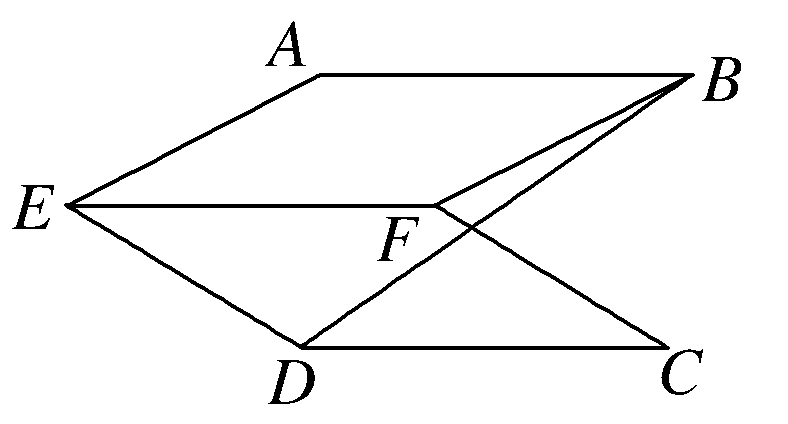
\includegraphics[width=86mm,alt={@@@494a628b97d74c2894c135f69e8f1eb7}]{media/media/image4.png}

A．\(\sqrt{3}\)；B．\(\sqrt{2}\)；C．1；D．\(\sqrt{3 - \sqrt{2}}\)

\noindent\biaoqian{【答案】}\ansbox{D}\quad\biaoqian{【知识点】}1.1.1 空间向量数量积的应用

\biaoqian{【分析】}由\(\overrightarrow{DB} = \overrightarrow{ED} + \overrightarrow{FE} + \overrightarrow{BF}\)，利用数量积运算性质展开即可得到答案

\biaoqian{【详解】}\(\because\overrightarrow{BD} = \overrightarrow{ED} + \overrightarrow{FE} + \overrightarrow{BF}\),\(\therefore\left| \overrightarrow{BD} \right|^{2} = \left| \overrightarrow{BF} \right|^{2} + \left| \overrightarrow{FE} \right|^{2} + \left| \overrightarrow{ED} \right|^{2} + 2\overrightarrow{BF} \bullet \overrightarrow{FE} + 2\overrightarrow{FE} \bullet \overrightarrow{ED} + 2\overrightarrow{BF} \bullet \overrightarrow{ED} = 1 + 1 + 1 - \sqrt{2}\)故\(\left| \overrightarrow{BD} \right| = \sqrt{3 - \sqrt{2}}\)故选\(D\)

\biaoqian{【点睛】}本题是要求空间两点之间的距离，运用空间向量将其表示，然后计算得到结果，较为基础．

\zutit{1.1.1.10 数量积求距离（折叠矩形）}

1题：-10

\biaoqian{【编注】}题型通式：题干为平面图形沿一条直线折起且折后两面垂直、求两点间距离时，判归本题型。第一步在折后图形中过两点向折痕作垂线定出垂足；再把目标向量写成两段垂线与折痕段的和链并平方展开；最后利用面面垂直带来的向量垂直逐项化简、开方得距离。

\timu{1.1.1.10-10．（中档）}{已知矩形\(ABCD\)中，\(AB = 1\)，\(BC = \sqrt{3}\)，将矩形\(ABCD\)沿对角线\(AC\)折起，使平面\(ABC\)与平面\(ACD\)垂直，则\(|\overrightarrow{BD}| =\)（~~~~）．}

A．\(\frac{\sqrt{10}}{2}\)；B．\(\frac{\sqrt{6}}{2}\)；C．\(\frac{\sqrt{5}}{2}\)；D．2

\noindent\biaoqian{【答案】}\ansbox{A}\quad\biaoqian{【知识点】}1.1.1 空间向量数量积的应用

\biaoqian{【分析】}过点\(B\)，\(D\)分别向\(AC\)作垂线，垂足分别为\(M\)，\(N\)，由\(\overrightarrow{BD} = \overrightarrow{BM} + \overrightarrow{MN} + \overrightarrow{ND}\)，平方后结合长度和垂直关系可得解.

\biaoqian{【详解】}
\includegraphics[width=45mm,alt={@@@e34e5148-bca3-440e-84b1-3cbf33fe2cc1}]{media/media/image5.png}~~过点\(B\)，\(D\)分别向\(AC\)作垂线，垂足分别为\(M\)，\(N\)，则可得\(AM = \frac{1}{2}\)，\(BM = \frac{\sqrt{3}}{2}\)，\(CN = \frac{1}{2}\)，\(DN = \frac{\sqrt{3}}{2}\)，\(MN = 1\)．由于\(\overrightarrow{BD} = \overrightarrow{BM} + \overrightarrow{MN} + \overrightarrow{ND}\)，所以\(|\overrightarrow{BD}|^{2} = {(\overrightarrow{BM} + \overrightarrow{MN} + \overrightarrow{ND})}^{2}\)\(= |\overrightarrow{BM}|^{2} + |\overrightarrow{MN}|^{2} + |\overrightarrow{ND}|^{2} + 2(\overrightarrow{BM} \cdot \overrightarrow{MN} + \overrightarrow{MN} \cdot \overrightarrow{ND} + \overrightarrow{BM} \cdot \overrightarrow{ND})\)\(= \left( \frac{\sqrt{3}}{2} \right)^{2} + 1^{2} + \left( \frac{\sqrt{3}}{2} \right)^{2} + 2 \times (0 + 0 + 0) = \frac{5}{2}\)，所以\(|\overrightarrow{BD}| = \frac{\sqrt{10}}{2}\)．故选:\emph{A}．

\biaoqian{【点睛】}本题主要考查了空间向量数量积的应用，属于基础题.
